%! Author = TiagoRG
%! GitHub = https://github.com/TiagoRG

\documentclass{report}
\usepackage[T1]{fontenc} % Fontes T1
\usepackage[utf8]{inputenc} % Input UTF8
\usepackage[backend=biber, style=ieee]{biblatex} % para usar bibliografia
\usepackage{csquotes}
\usepackage[english]{babel}
\usepackage{blindtext} % Gerar texto automaticamente
\usepackage[printonlyused]{acronym}
\usepackage{hyperref} % para autoref
\usepackage{graphicx}
\usepackage{indentfirst}
\usepackage{float}
\usepackage{fancyhdr}
\usepackage{geometry}
\usepackage{listings}
\usepackage{array}
\usepackage{tabularx}
\renewcommand{\familydefault}{\sfdefault}
\newcolumntype{Y}{>{\centering\arraybackslash}X}
\newcolumntype{Z}{>{\centering\arraybackslash}m{1.1\dimexpr(\textwidth-20\tabcolsep)/9\relax}}
\newcolumntype{F}{>{\centering\arraybackslash}m{1.2\dimexpr(\textwidth-20\tabcolsep)/9\relax}}
\newcolumntype{S}{>{\centering\arraybackslash}m{0.35\dimexpr(\textwidth-20\tabcolsep)/9\relax}}
\newcolumntype{L}{>{\centering\arraybackslash}m{1.5\dimexpr(\textwidth-20\tabcolsep)/9\relax}}

\geometry{
    paper=a4paper,
    margin=45pt,
    includefoot
}

\begin{document}

\renewcommand{\headrulewidth}{0.5pt} % remove lines as well
\renewcommand{\footrulewidth}{0.5pt}
\fancypagestyle{plain}{
    \fancyhf{}% Clear header/footer
    \fancyhead[L]{
\includegraphics[width=25pt,height=25pt]{ua} Universidade de Aveiro}% Right header
    \fancyhead[R]{Departamento de Electrónica, Telecomunicações e Informática}% Right header
    \fancyfoot[L]{Rúben Gomes\\(113435) rlcg@ua.pt}% Left footer
    \fancyfoot[R]{Tiago Garcia\\(114184) tiago.rgarcia@ua.pt}% Right footer
}
\pagestyle{plain}

\chapter*{Nmecs}
Since our nmecs are 113435 and 114184, the list of numbers to be used in the IP addresses is the following:

\begin{itemize}
    \item \textbf{$X_1$} $\rightarrow$ 1
    \item \textbf{$X_2$} $\rightarrow$ 3
    \item \textbf{$X_3$} $\rightarrow$ 4
    \item \textbf{$X_4$} $\rightarrow$ 3
    \item \textbf{$X_5$} $\rightarrow$ 5
    \item \textbf{$X_6$} $\rightarrow$ 1
    \item \textbf{$X_7$} $\rightarrow$ 4
    \item \textbf{$X_8$} $\rightarrow$ 1
    \item \textbf{$X_9$} $\rightarrow$ 8
    \item \textbf{$X_0$} $\rightarrow$ 4
\end{itemize}

\chapter*{Private IPv4 Assignment}

\begin{table}[H!]
\centering
\caption{Private IPv4 assignment}

\begin{center}
\scriptsize
\begin{tabularx}{1\textwidth}{|Z|Z|Y|Y|Z|Z|Y|Y|Y|}
    \hline
    \multicolumn{9}{|c|}{\textbf{Private IPv4 assignment}} \\
    [0.5ex]
    \hline
    \hline
    & \textbf{Department} & Network ~~~~ Address & Mask & Broadcast ~~ Address & Available Addresses & Used Addresses & Gateway \#1 Address & Gateway \#2 Address \\

    \hline

    \multirow{\textbf{NewNet ISP}} & NewNetCenter & -- & -- & -- & -- & -- & -- & -- \\
    \cline{2-9}
    & NewNetIT & -- & -- & -- & -- & -- & -- & -- \\

    \hline

    \multirow{\textbf{Amazing}} & Offices & 10.54.76.0 & 23 & 10.54.77.255 & 10.54.76.3 $\rightarrow$ 10.54.77.254 & -- & 10.54.76.1 & 10.54.76.2 \\
    \cline{2-9}
    & WiFi & 10.54.72.0 & 22 & 10.54.75.255 & 10.54.72.3 $\rightarrow$ 10.54.75.254 & -- & 10.54.72.1 & 10.54.72.2 \\
    \cline{2-9}
    & Factory & 10.54.64.0 & 21 & 10.54.71.255 & 10.54.64.3 $\rightarrow$ 10.54.71.254 & -- & 10.54.64.1 & 10.54.64.2 \\
    \cline{2-9}
    & Interconnection Amazing - ESW\#1 & 10.54.78.0 & 30 & 10.54.78.3 & 10.54.78.1 $\rightarrow$ 10.54.78.2 & -- & -- & -- \\
    \cline{2-9}
    & Interconnection Amazing - ESW\#2 & 10.54.78.4 & 30 & 10.54.78.7 & 10.54.78.5 $\rightarrow$ 10.54.78.6 & -- & -- & -- \\

    \hline

    \multirow{\textbf{GR8}} & Office & 10.114.36.0 & 24 & 10.114.36.255 & 10.114.36.3 $\rightarrow$ 10.114.36.254 & -- & 10.114.36.1 & -- \\
    \cline{2-9}
    & WiFi & 10.114.37.0 & 24 & 10.114.37.255 & 10.114.37.3 $\rightarrow$ 10.114.37.254 & -- & 10.114.37.1 & -- \\

    \hline
\end{tabularx}
\end{center}

\end{table}

\subsection*{Justification}

\subsubsection*{NewNet ISP}
NewNet won't have any private IPv4 addresses assigned to it, since it is an ISP and it will only provide internet access to the other companies.

\subsubsection*{Amazing}
Starting off with the base address, this will be $10.0X_5X_0.64.0/20$, or $10.54.64.0/20$ when replacing with the nmec separation.

The Amazing Factory will take most of the addresses, so when dividing the network, it will have the addresses from $10.54.64.0/21$ to $10.54.71.255/21$ and will result on having $10.54.72.0/21$ to divide for the rest of the company. After the factory, WiFi is the one taking the most addresses so after dividing the resultant, it will be taking from $10.54.72.0/22$ to $10.54.75.255/22$ and resulting on $10.54.76.0/22$ to be divided once again for the offices. When doing so, they will be taking the addresses from $10.54.76.0/23$ to $10.54.77.255/23$ and leaving $10.54.78.0/23$ for the switches.

Since we want /30 sub-networks for the switches, and can still populate from $10.54.78.0$ to $10.54.79.255$, we will be using $10.54.78.0/30$ for AmazingL3SW1 and $10.54.78.4/30$ for AmazingL3SW2 resulting in 2 gateways for the Amazing network.

All this explained more visually in the following image.

\begin{figure}[H]
    \centering
    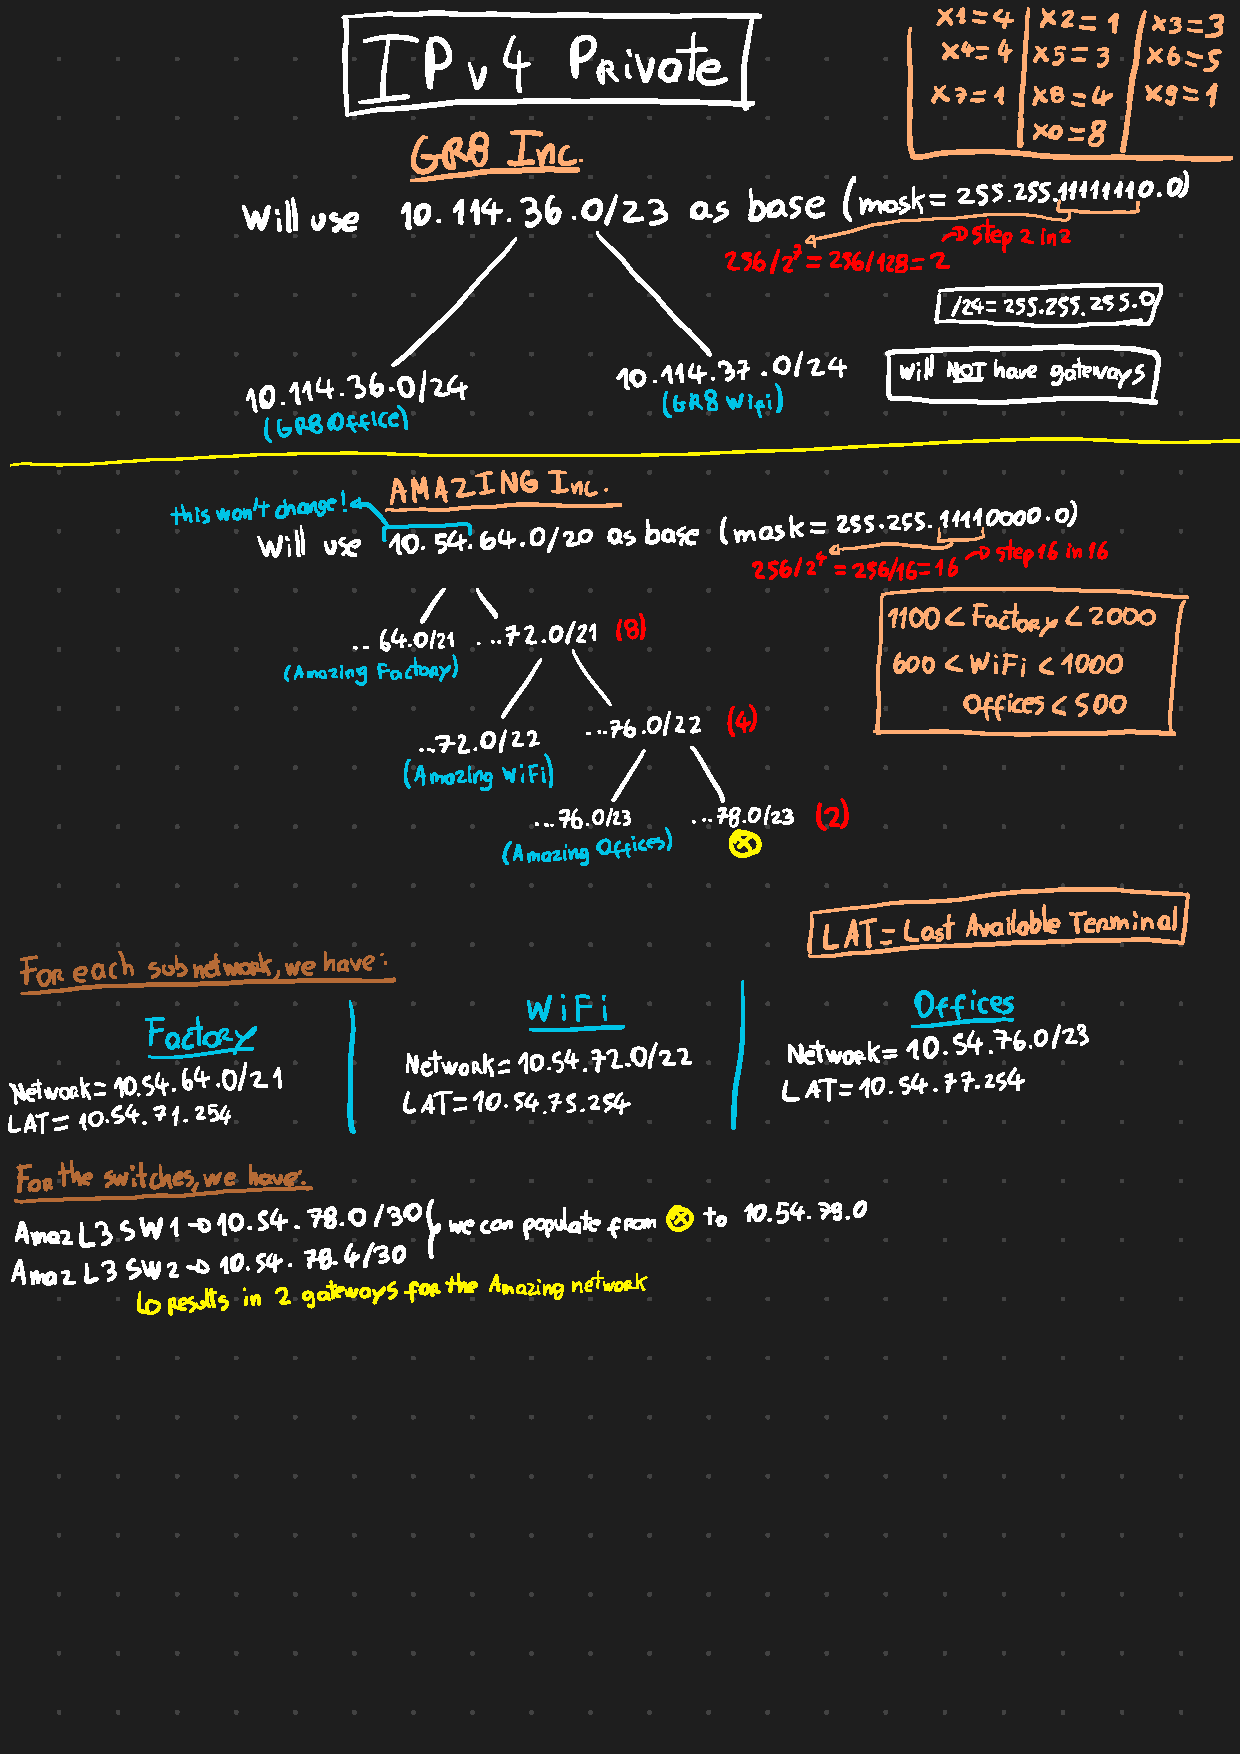
\includegraphics[width=\textwidth,trim={0 7cm 0 7.9cm},clip]{private-ipv4}
    \caption{Private IPv4 assignment for Amazing}
    \label{fig:private-ipv4-amazing}
\end{figure}

\subsubsection*{GR8}
GR8 will only have 2 networks, one for the office and one for the WiFi. The base address for this company will be $10.1X_8X_7.0X_46.0/23$ or $10.114.36.0/23$ when replacing the nmec numbers.

The office will be taking $10.114.36.0/24$ and the WiFi will be taking $10.114.37.0/24$.

This company will have no gateways.

\begin{figure}[H]
    \centering
    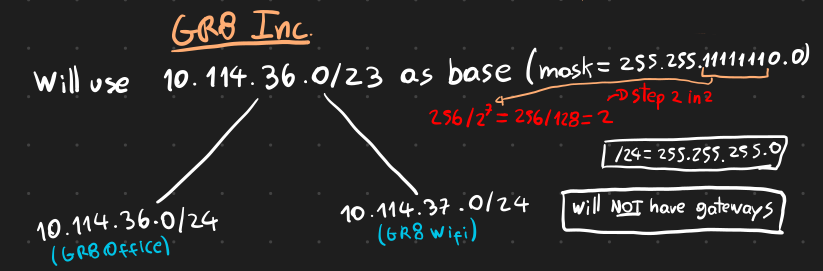
\includegraphics[width=\textwidth]{private-ipv4-gr8.png}
    \caption{Private IPv4 assignment for GR8}
    \label{fig:private-ipv4-gr8}
\end{figure}

\chapter*{Public IPv4 Assignment}

\begin{table}[H!]
\centering
\caption{Public IPv4 assignment}
\label{tab:public-ipv4-assignment}

\begin{center}
\scriptsize
\begin{tabularx}{1\textwidth}{|F|Z|Z|S|Z|Z|Y|Z|Y|}
    \hline
    \multicolumn{9}{|c|}{\textbf{Public IPv4 assignment}} \\
    [0.5ex]
    \hline
    \hline
    & \textbf{Department} & Network Address & Mask & Broadcast Address & Available Addresses & Used Addresses & Gateway \#1 Address & Gateway \#2 Address \\

    \hline

    \multirow{\textbf{NewNet ISP}} & NewNetCenter & 201.134.15.128 & 26 & 201.134.15.191 & 201.134.15.130 $\rightarrow$ 201.134.15.190 & -- & 201.135.15.129 & -- \\
    \cline{2-9}
    & NewNetIT & 201.134.15.96 & 27 & 201.134.15.127 & 201.134.15.98 $\rightarrow$ 201.134.15.126 & -- & 201.135.15.97 & -- \\

    \hline

    \multirow{\textbf{Amazing}} & Offices & 201.134.15.192 & 26 & 201.134.15.255 & 201.134.15.195 $\rightarrow$ 201.134.15.254 & -- & 201.135.15.193 & 201.135.15.194 \\
    \cline{2-9}
    & WiFi & -- & -- & -- & -- & -- & -- & -- \\
    \cline{2-9}
    & Factory & -- & -- & -- & -- & -- & -- & -- \\
    \cline{2-9}
    & NAT/PAT & 201.134.15.32 & 27 & 201.134.15.61 & 201.134.15.33 $\rightarrow$ 201.134.15.60 & -- & -- & -- \\

    \hline

    \multirow{\textbf{GR8}} & Office & 201.134.15.64 & 27 & 201.134.15.95 & 201.134.15.66 $\rightarrow$ 201.134.15.94 & -- & 201.135.15.65 & -- \\
    \cline{2-9}
    & WiFi & -- & -- & -- & -- & -- & -- & -- \\
    \cline{2-9}
    & NAT/PAT & 201.134.15.16 & 28 & 201.134.15.31 & 201.134.15.17 $\rightarrow$ 201.134.15.30 & -- & -- & -- \\

    \hline

    \multirow{\textbf{Interconnection}} & NewNet - Amazing & 201.134.15.8 & 30 & 201.134.15.11 & 201.134.15.9 $\rightarrow$ 201.134.15.10 & -- & -- & -- \\
    \cline{2-9}
    & NewNet - GR8 & 201.134.15.12 & 30 & 201.134.15.15 & 201.134.15.13 $\rightarrow$ 201.134.15.14 & -- & -- & -- \\

    \hline
\end{tabularx}
\end{center}

\end{table}

\subsection*{Justification}

The base public address for this assignment will be $20X_1.1X_2X_0.0X_6X_5.0/24$ or $201.134.15.0/24$ when replacing the nmec numbers. This means we will have a total of 256 addresses to use.

Since we only have one ISP, we will need to divide the same network for all the companies in order to meet all the following requirements:

\begin{itemize}
    \item 60 addresses for Amazing Offices
    \item 50 addresses for NewNet Center
    \item 16 addresses for NewNet IT
    \item 22 addresses for GR8 Office
    \item 20 addresses for Amazing NAT/PAT
    \item 9 addresses for GR8 NAT/PAT
\end{itemize}

\begin{figure}
    \centering
    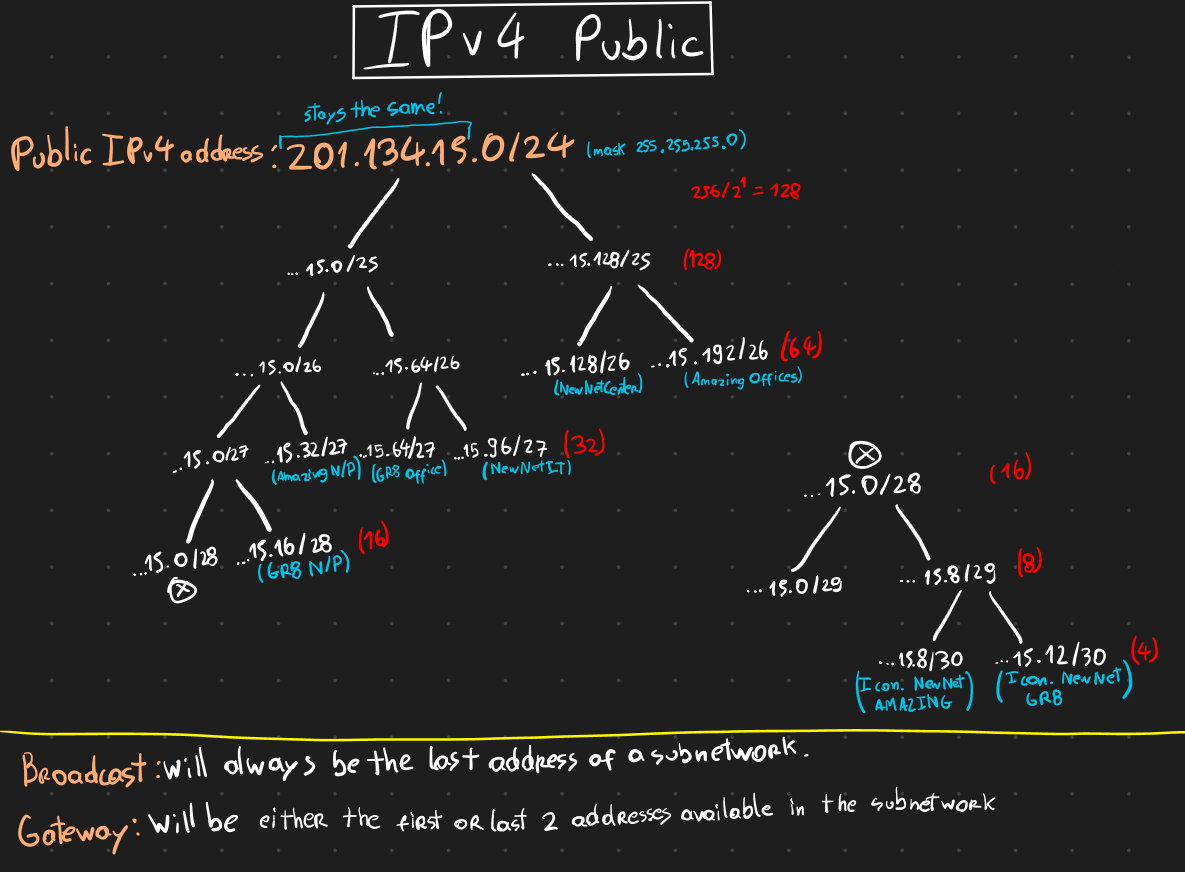
\includegraphics[width=\textwidth,trim={0 14cm 0 0},clip]{public-ipv4}
    \caption{Public IPv4 assignment}
    \label{fig:public-ipv4}
\end{figure}


\chapter*{Global IPv6 Assignment}

\begin{table}[H!]
    \centering

    \begin{center}
    \scriptsize

    \begin{tabularx}{1\textwidth}{|F|Z|Z|Y|L|L|Z|Z|}
        \hline
        \multicolumn{8}{|c|}{\textbf{Global IPv6 assignment}} \\
        [0.5ex]
        \hline
        \hline
        & \textbf{Department} & Network Address & Mask & Available Addresses & Used Addresses & Gateway \#1 Address & Gateway \#2 Address \\

        \hline

        \multirow{\textbf{NewNet ISP}} & NewNetCenter & \textbf{G}:11C0:: & 64 & \textbf{G}:11C0::0002 $\rightarrow$ \textbf{G}:11C0:FFFF:FFFF & -- & \textbf{G}:11C0::0001 & -- \\
        \cline{2-8}
        & NewNetIT & \textbf{G}:11C1:: & 64 & \textbf{G}:11C1::0002 $\rightarrow$ \textbf{G}:11C1:FFFF:FFFF & -- & \textbf{G}:11C1::0001 & -- \\

        \hline

        \multirow{\textbf{Amazing}} & Offices & \textbf{G}:1180:: & 64 & \textbf{G}:1180::0003 $\rightarrow$ \textbf{G}:1180:FFFF:FFFF & -- & \textbf{G}:1180::0001 & \textbf{G}:1180::0002 \\
        \cline{2-8}
        & WiFi & \textbf{G}:1181:: & 64 & \textbf{G}:1181::0003 $\rightarrow$ \textbf{G}:1181:FFFF:FFFF & -- & \textbf{G}:1181::0001 & \textbf{G}:1181::0002 \\
        \cline{2-8}
        & Factory & -- & -- & -- & -- & -- & -- \\
        \cline{2-8}
        & Interconnection Amazing - ESW\#1 & FE80:: & 10 & FE80::1 & -- & -- & -- \\
        \cline{2-8}
        & Interconnection Amazing - ESW\#2 & FE80:: & 10 & FE80::2 & -- & -- & -- \\

        \hline

        \multirow{\textbf{GR8}} & Office & \textbf{G}:1190:: & 64 & \textbf{G}:1190::0002 $\rightarrow$ \textbf{G}:1190:FFFF:FFFF & -- & \textbf{G}:1190::0001 & -- \\
        \cline{2-8}
        & WiFi & \textbf{G}:1191:: & 64 & \textbf{G}:1191::0002 $\rightarrow$ \textbf{G}:1191:FFFF:FFFF & -- & \textbf{G}:1191::0001 & -- \\

        \hline

        \multirow{\textbf{Interconnection}} & NewNet - Amazing & \textbf{G}:1100::0002 & 126 & \textbf{G}:1100::0002 $\rightarrow$ \textbf{G}:1100::0003 & -- & \textbf{G}:1100::0001 & -- \\
        \cline{2-8}
        & NewNet - GR8 & \textbf{G}:1100::0004 & 126 & \textbf{G}:1100::0006 $\rightarrow$ \textbf{G}:1100::0007 & -- & \textbf{G}:1100::0005 & -- \\

        \hline
    \end{tabularx}

    \caption{Global prefix: \textbf{G} = 2002:8888:4314}

    \end{center}
\end{table}

\pagebreak
\subsection*{Justification}

Our global IPv6 prefix will be 2002:8888:4314:1100::/56. From there, we will divide it into all the subnets we need as explained in the following image.

\begin{figure}[H]
    \centering
    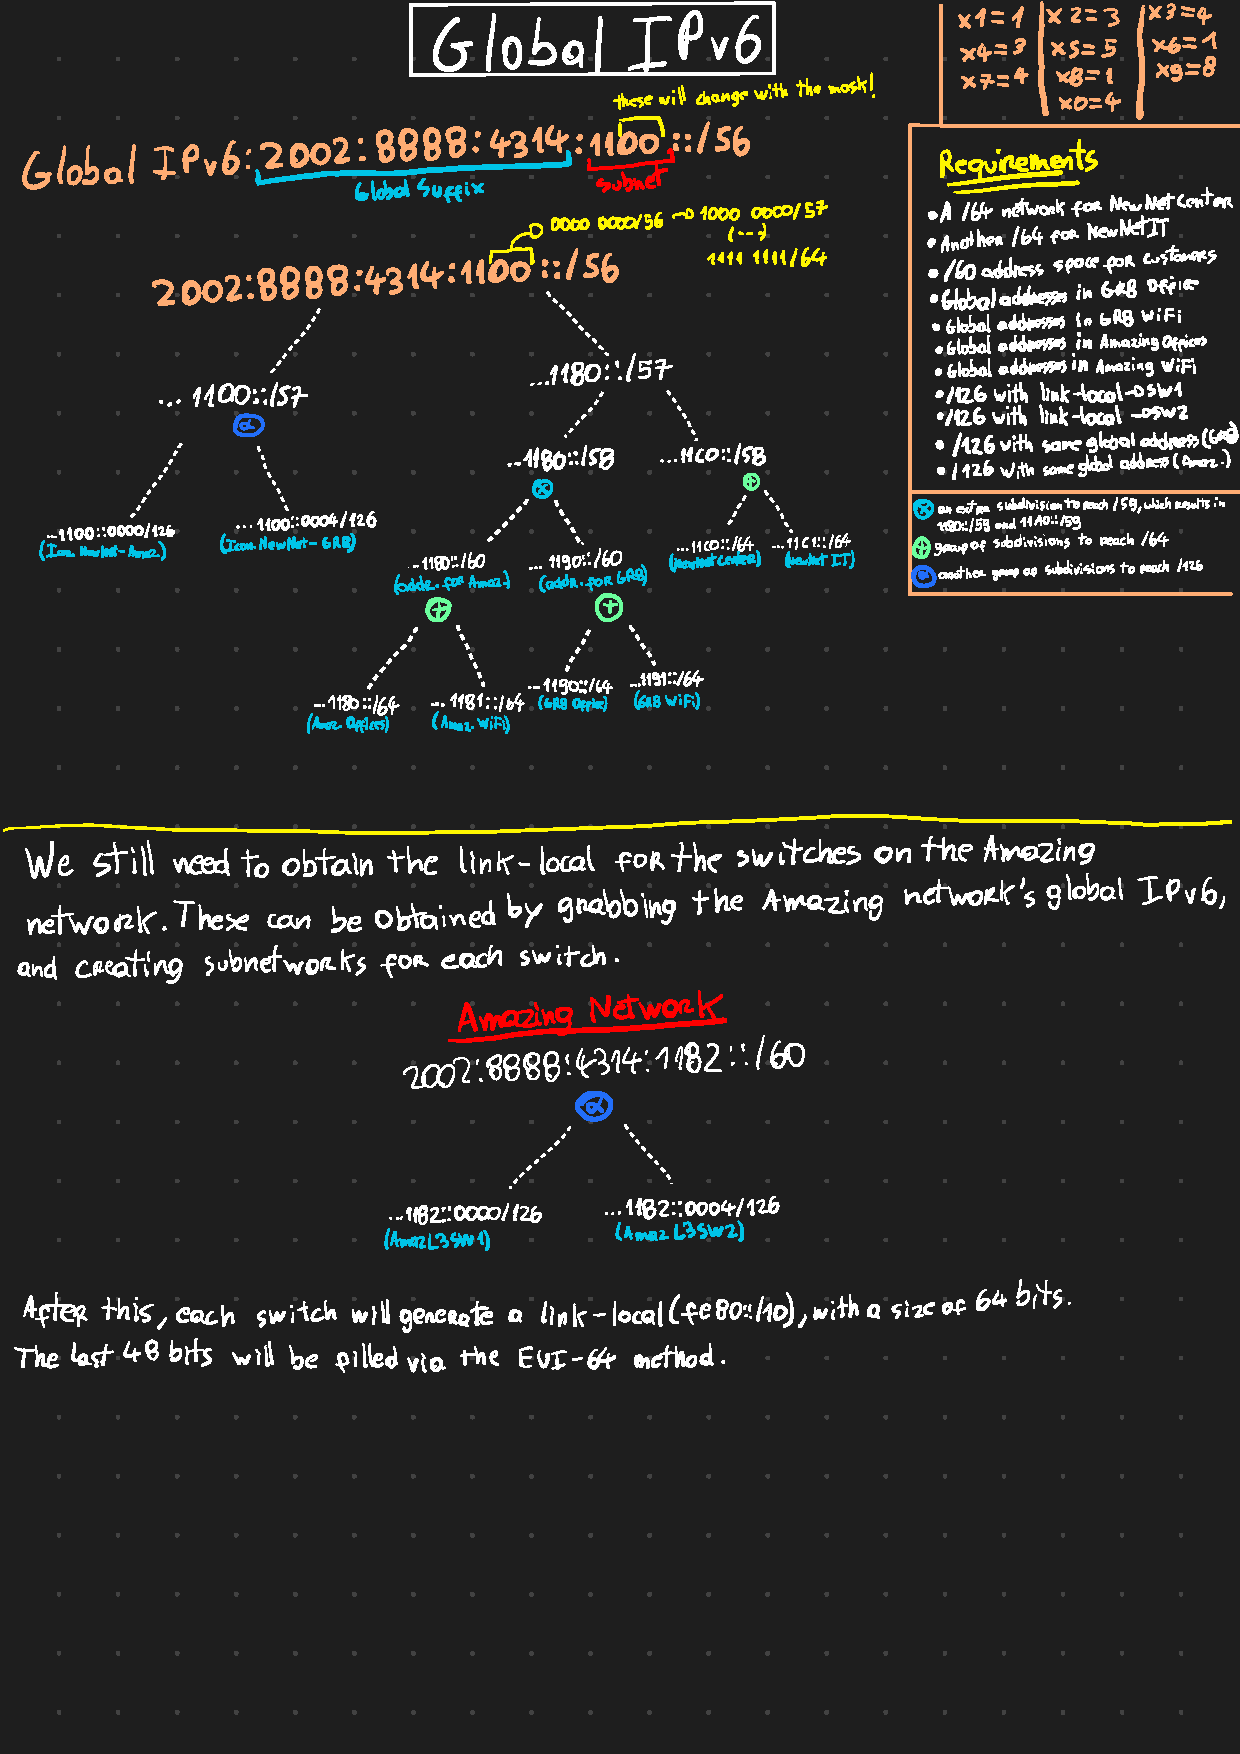
\includegraphics[width=\textwidth,trim={0 6cm 0 0},clip]{global-ipv6}
    \caption{Global IPv6 assignment}
    \label{fig:global-ipv6}
\end{figure}

\end{document}
